\newcommand{\teststatus}{Pianificato}

\section {Pianificazione dei test}

Si descrivono di seguito tutti i test di validazione, sistema ed integrazione previsti, prevedendo un aggiornamento futuro per i test di unità. Per le tempistiche di esecuzione dei test si faccia riferimento al \textit{Piano di Progetto} v2.0. Nelle tabelle sottostanti lo stato dei test "Pianificato" è da intendersi come non applicato in quanto tali test saranno applicati successivamente, come descritto nel \textit{Piano di Progetto}.

\subsection {Test di sistema}

In questa sezione vengono descritti i test di sistema che permettono di verificare il comportamento dinamico del sistema completo rispetto ai requisiti descritti nell’\textit{Analisi dei Requisiti v2.0}.
I test di sistema riportati sono quelli relativi ai requisiti software individuati e pertanto meritevoli di un test.

\subsubsection{Descrizione dei test di sistema}

\begin{longtable}{|l|p{2.5cm}|p{5cm}|p{3.5cm}|}
\hline
\textbf{Requisito} & \textbf{Stato} & \textbf{Descrizione} & \textbf{Test} \\
\hline
FOb1 & \teststatus & Si verifica che il sistema permetta  la creazione di una presentazione e che questa venga effettivamente creata e salvata sul database & TS1\\
\hline
FOb3 & \teststatus & Si testa l'esecuzione di una presentazione, verificando che il percorso seguito sia quello scelto dall'utente ed il corretto avanzamento delle slides& TS3\\
\hline
FOb3.5 & \teststatus & Si verifica il funzionamento dei checkpoint, la possibilità per l'utente di impostare un checkpoint e il corretto funzionamento dei percorsi di approfondimento & TS3.5  \\
\hline
FOb4 & \teststatus  & Si verifica che le modifiche apportate dall'utente ad una presentazione, quali ad esempio inserimento di oggetti grafici, testi o nuovi frame vengano correttamente applicate e salvate dal sistema & TS4 \\
\hline
FOb5 & \teststatus  & Viene verificato che il salvataggio della presentazione avvenga con successo e nel formato atteso & TS5 \\
\hline
FOb6 & \teststatus & Si verifica che l'azione di eliminazione da parte di un'utente di una presentazione cancelli effettivamente tutti i dati relativi a quella presentazione dal sistema & TS6 \\
\hline
FOb6.1 & \teststatus  & Si testa l'annullamento del comando di eliminazione e si verifica che non vi sia alcuna modifica alla presentazione fintanto che l'azione non viene confermata al sistema dall'utente. & TS6.1 \\
\hline
FOb7 & \teststatus & Si verifica che il sistema permetta la pubblicazione di una presentazione e che questa vada a buon fine & TS7 \\
\hline
FOb8 & \teststatus  & Il sistema deve poter generare un link per una presentazione live & TS8 \\
\hline
FOp9 & \teststatus  & l'utente deve poter rendere privata una presentazione pubblica & TS9 \\
\hline
FOb11.1 & \teststatus  & Viene verificato che il sistema permetta di esportare la presentazione in formato poster controllando che il file di output corrisponda alla presentazione esportata &  TS11.1 \\
\hline
FOb11.2 & \teststatus & Si verifica che il formato con cui viene esportata la presentazione sia portabile & TS11.2 \\
\hline
FOb13 & \teststatus  & Si verifica che il sistema permetta all'utente di registrarsi simulando i passi della procedura di registrazione e successivamente verificando il salvataggio dei dati inseriti dall'utente & TS13
\\
\hline
FOb14 & \teststatus  & Si verifica che il sistema permetta all'utente di autenticarsi & TS14 \\
\hline
FOb15 & \teststatus  & Viene verificato il corretto funzionamento di tutti i messaggi di errore da parte del sistema  l'utente deve sapere quando ha commesso un errore & TS15\\
\hline
FOb16 & \teststatus  & Viene verificata e provata la procedura di cambio password, assicurandosi che il sistema salvi correttamente le modifiche dell'utente& TS16\\
\hline
VOb17 & \teststatus  & Viene testato l'avvio del sistema su browser Chrome da versione 40+& TS17\\
\hline
\caption{Tabella di tracciamento test di sistema / requisiti}
	
\end{longtable}
\newpage
\subsection {Test di integrazione}

In questa sezione vengono descritti i test di integrazione per i vari componenti descritti nella progettazione ad alto livello, che permettono di verificare la corretta integrazione ed il corretto flusso dei dati all'interno del sistema. Si è scelta una strategia di integrazione incrementale, il cui principale vantaggio è quello di poter sviluppare e verificare le componenti in parallelo.
Con l'approccio incrementale, infatti, i difetti rilevati da un test sono da attribuirsi, con maggior probabilità, all'ultima componente aggiunta ed essendo ogni passo di integrazione reversibile è possibile retrocedere ed effettuare un rollback ad uno stato noto e sicuro.
Per i test di integrazione è stato utilizzato il metodo bottom-up, questa scelta risulta automatica avendola già adottata nella progettazione delle componenti con l'obiettivo quello di ridurre le dipendenze funzionali di ogni singola componente.
Il diagramma seguente non rispetta il formalismo UMLG 2.x ed è utilizzato per semplificare l'illustrazione della strategia di integrazione. Si possono notare, lungo l'albero, dei macro componenti che possono integrare al loro interno due o più componenti di maggior dettaglio.

\begin{figure}[h!]
	\centering
	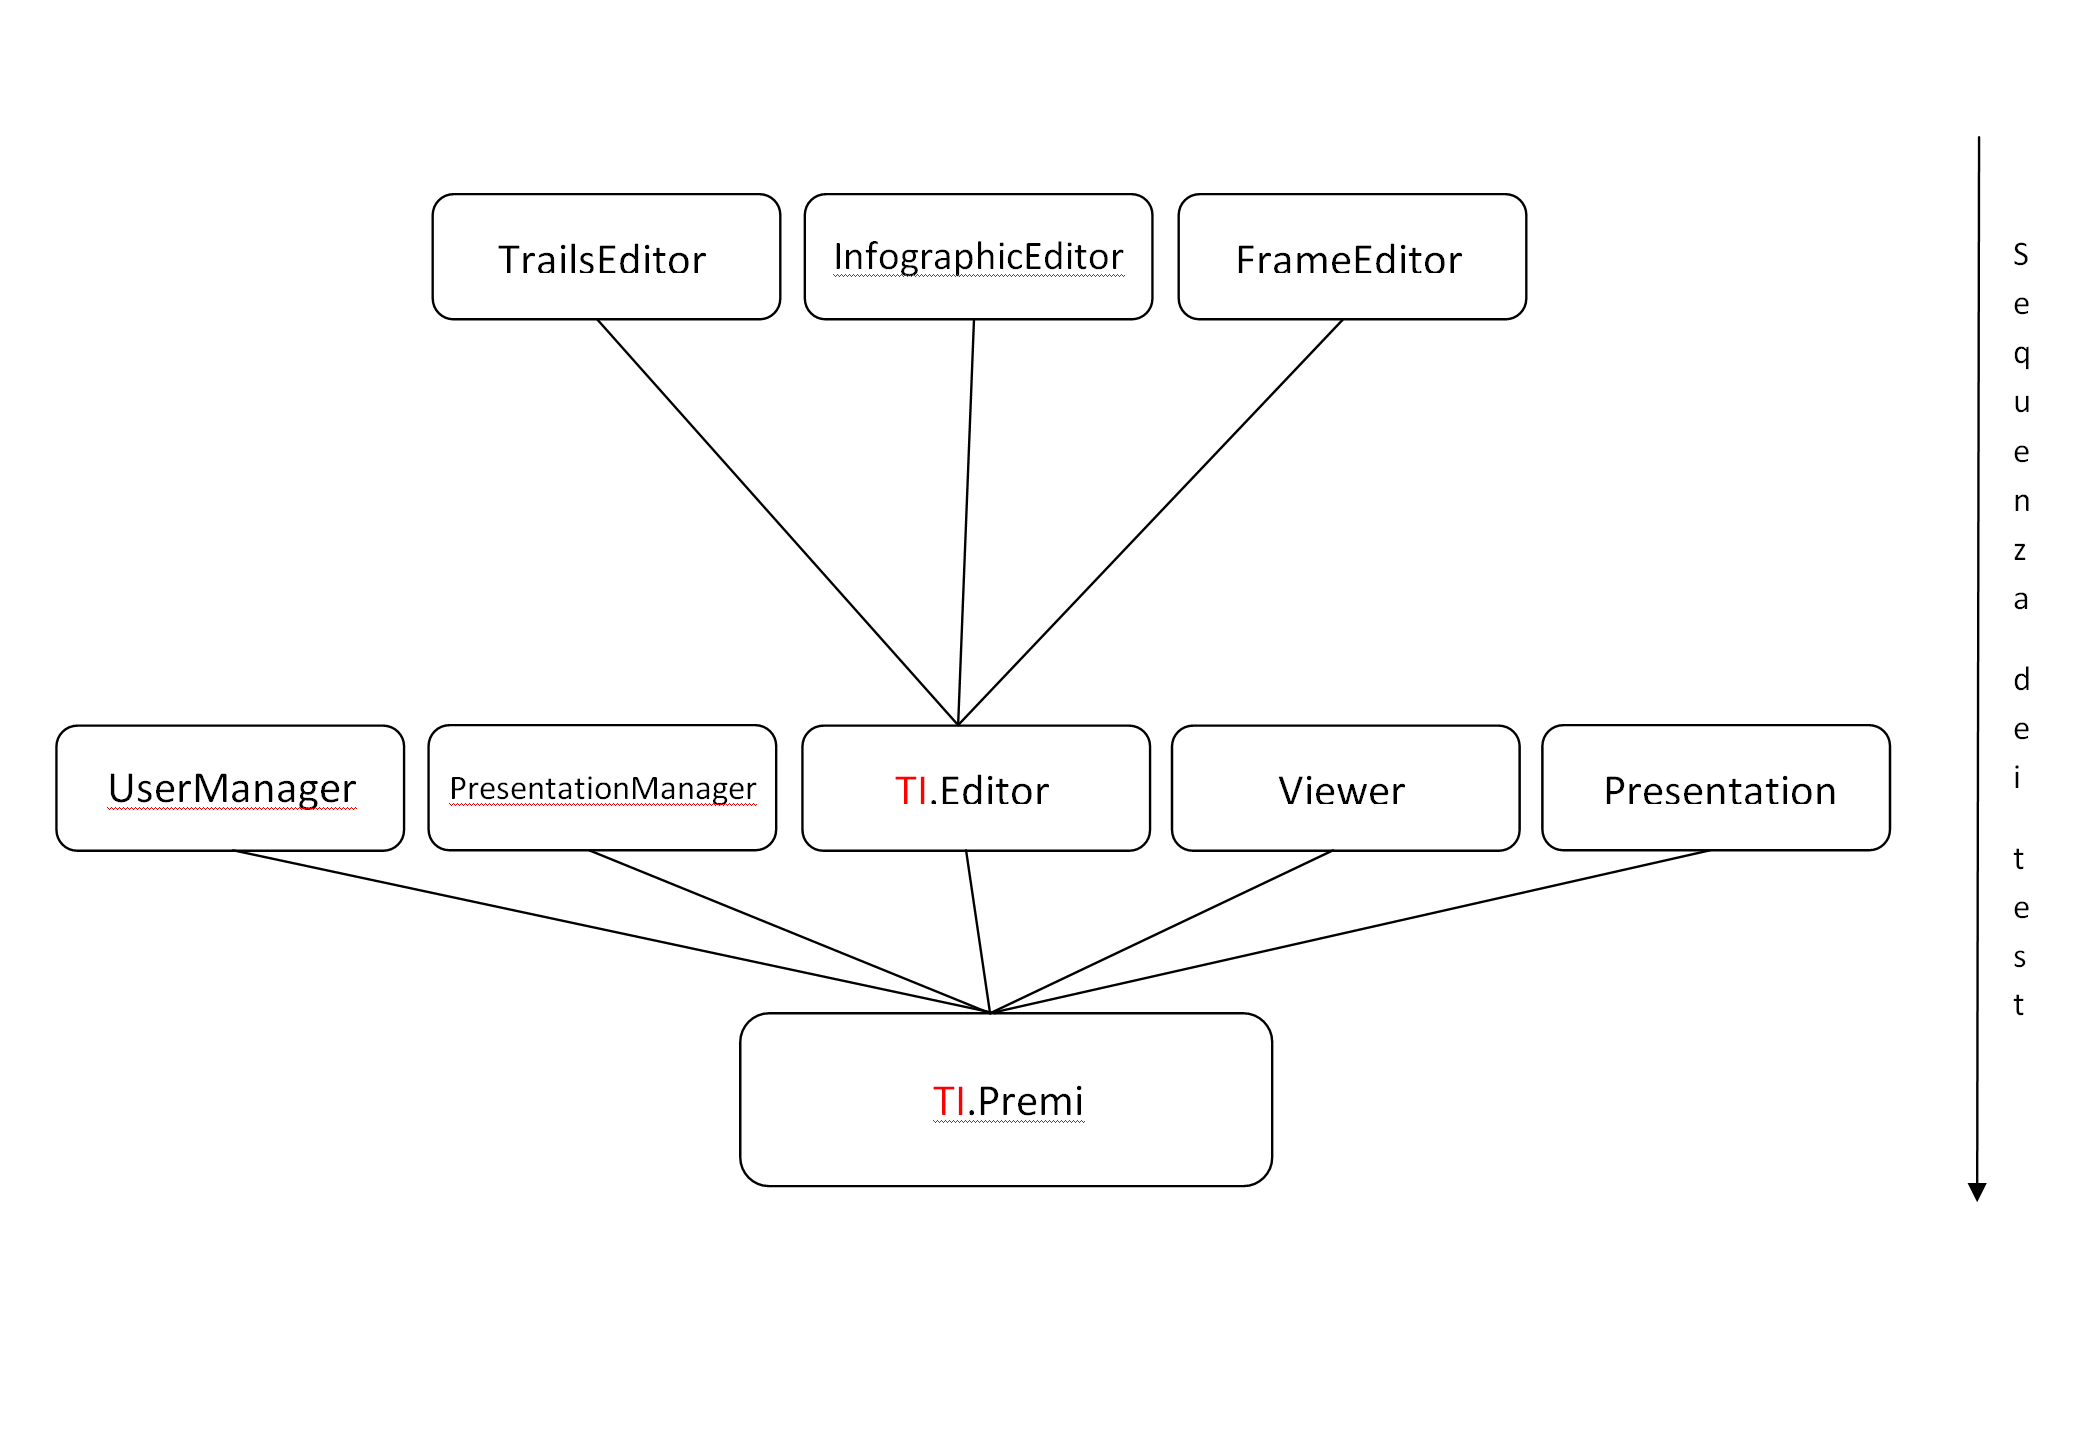
\includegraphics[scale=.45]{img/integrationTests.png}
	\caption{Diagramma informale della strategia di integrazione}
	\label{fig:Diagramma informale della strategia di integrazione}
\end{figure}
\newpage
\subsubsection{Descrizione dei test di integrazione}

\begin{longtable}{|p{4.5cm}|p{7cm}|p{2.5cm}|}
	\hline
	\textbf{Test} & \textbf{Descrizione} & \textbf{Stato} \\
	\hline
	TI.Premi & Test di integrazione finale per le componenti del modulo Premi & \teststatus \\
	\hline
	TI.UserManager & \textbf{Gestione dell'Utente}: Verifica il corretto funzionamento delle operazioni di registrazione, autenticazione e cambio password & \teststatus \\
	\hline
	TI.PresentationManager & \textbf{Gestione della presentazione}: Verifica il corretto funzionamento del sistema di gestione della presentazione, testa la correttezza delle operazioni di creazione, modifica eliminazione, pubblicazione, esportazione e portabilità di una presentazione& \teststatus \\
	\hline
	TI.Editor & Test di integrazione finale per le componenti del modulo Premi::Editor & \teststatus \\
	\hline
	TI.TrailsEditor & \textbf{Edit dei percorsi}: Verifica il corretto funzionamento dei percorsi, e le procedure di creazione, modifica, clonazione ed eliminazione di un persorso & \teststatus \\
	\hline
	TI.InfographicEditor & \textbf{Edit dell'Infografica}: Verifica il corretto funzionamento delle infografiche, nello specifico l'aggiunta di frame, immagini, testi e shape all'infografica e la modifica dello stile& \teststatus \\
	\hline
	TI.FrameEditor & \textbf{Edit dei Frame}: Verifica il corretto funzionamento dei frame, nello specifico l'aggiunta di immagini, testi e shape al frame e la modifica dello stile & \teststatus \\
	\hline
	TI.Viewer & \textbf{Visualizzazione della presentazione}: Verifica la corretta riproduzione della presentazione& \teststatus \\
	\hline
	\caption{Tabella test di integrazione}
\end{longtable}

\subsubsection{Tracciamento componenti – test di integrazione}

%bla bla

\begin{longtable}{|l|l|}
	\hline
	\textbf{Componente} & \textbf{Test} \\
	\hline
	Premi & TI.Premi \\
	\hline
	Premi::UserManager & TI.UserManager \\
	\hline
	Premi::UserManager::Views & Architettura del Sistema \\
	\hline
	Premi::UserManager::Controllers & Architettura del Sistema \\
	\hline
	Premi::PresentationManager & TI.PresentationManager \\
	\hline
	Premi::PresentationManager::Views & Architettura del Sistema \\
	\hline
	Premi::PresentationManager::Controllers & Architettura del Sistema \\
	\hline
    Premi::Editor & TI.Editor \\
    \hline
	Premi::Editor::Views & Architettura del Sistema \\
	\hline
	Premi::Editor::Controllers & Architettura del Sistema \\
	\hline
	Premi::Editor::TrailsEditor & TI.TrailsEditor \\
	\hline
	Premi::Editor::TrailsEditor::Views & Architettura del Sistema \\
    \hline
    Premi::Editor::TrailsEditor::Controllers & Architettura del Sistema \\
	\hline
	Premi::Editor::InfographicEditor & TI.InfographicEditor\\
    \hline
    Premi::Editor::InfographicEditor::Views & Architettura del Sistema \\
    \hline
    Premi::Editor::InfographicEditor::Controllers & Architettura del Sistema \\
   	\hline
   	Premi::Editor::FrameEditor & TI.FrameEditor\\
   	\hline
   	Premi::Editor::FrameEditor::Views & Architettura del Sistema \\
   	\hline
   	Premi::Editor::FrameEditor::Controllers & Architettura del Sistema \\
   	\hline
   	Premi::Viewer & TI.Viewer\\
   	\hline
   	Premi::Viewer::Views & Architettura del Sistema \\
   	\hline
   	Premi::Viewer::Controllers & Architettura del Sistema \\
    \hline
	\caption{Tabella tracciamento componente - test di integrazione}
\end{longtable}



\subsection {Test di validazione}

In questa sezione vengono descritti i test di validazione che servono per accertarsi che il prodotto realizzato sia conforme alle attese.
Per ogni test vengono descritti i vari passi che un utente deve eseguire per testare i requisiti ad esso associati.

\subsubsection {Test TV1} %registrazione
L'utente vuole verificare che ci si possa registrare al sistema Premi.\\
All'utente è richiesto di:
\begin{itemize}
	\item Aprire il sistema
	\item Navigare nell'area di registrazione
	\item Inserire un indirizzo email. \\
	         All'utente è chiesto di: 
	         \begin{itemize}
	         	\item Verificare che l'inserimento di un indirizzo email non valido generi un avviso da parte del sistema
	         	\item Inserire un indirizzo email valido
	         \end{itemize}
	\item Inserire una password
	\item Reinserire la password per conferma
	\item Verificare che il completamento della registrazione al sistema vada a buon fine
\end{itemize}

\subsubsection {Test TV2} %autenticazione
L'utente vuole verificare il corretto funzionamento dell'autenticazione al sistema Premi\\
All'utente è richiesto di:
\begin{itemize}
	\item Eseguire la registrazione al sistema Premi eseguendo \textbf{TV1}.
	\item Accedere alla sezione di Login del sistema Premi
	\item Inserire un indirizzo email \\
		All'utente è chiesto di: 
		\begin{itemize}
			\item Verificare che l'inserimento di un indirizzo email non valido generi un avviso da parte del sistema
			\item Provare l'inserimento di un indirizzo email diverso da quello fornito in fase di registrazione
		\end{itemize}
	\item Inserire una password\\
	All'utente è chiesto di: 
			\begin{itemize}
				\item Provare l'inserimento di una password diversa da quella fornita in fase di registrazione
				\item Testare la procedura guidata di cambio password (\textbf{TV2.1})
			\end{itemize}
	\item Verificare che in caso di indirizzo mail o password diversi da quelli forniti in fase di registrazione generi un messaggio di errore non facendo terminare a buon fine l'autenticazione.
	\item Verificare che l'autenticazione vada a buon fine e il sistema renda esplicito il successo di questa azione.
\end{itemize}
	 
\subsubsection {Test TV3} % creazione e eliminazione di una presentazione nuova

L'utente vuole testare la creazione di una nuova presentazione e successivamente la sua eliminazione\\
All'utente è richiesto di:
\begin{itemize}
	\item Autenticarsi al sistema Premi eseguendo \textbf{TV2}
	\item Creare una nuova presentazione 
	\item Scegliere ed inserire un titolo per la nuova presentazione (\textbf{TV.3.1}) 
	\item Scrivere una descrizione di almeno di almeno 15 parole per la presentazione (\textbf{TV.3.2})  
	\item Completare la procedura di creazione confermando i dati inseriti
	\item Constatare l'avvenuta creazione della presentazione
	\item Selezionare la presentazione
	\item Eliminare la presentazione selezionata 
	\item Annullare l'operazione di eliminazione prima che questa avvenga effettivamente (\textbf{TV.3.3})
\end{itemize}

\subsubsection {Test TV4} % esecuzione di una presentazione navigazione

L'utente vuole testare l'esecuzione di una presentazione\\
All'utente è richiesto di:

\begin{itemize}
	\item Autenticarsi al sistema Premi eseguendo \textbf{TV2}
	\item Selezionare una presentazione dall'elenco delle presentazioni (\textbf{TV4.1}) 
	\item Scegliere un percorso per la presentazione tra quelli disponibili (\textbf{TV4.2})
	\item Navigare nella presentazione:\\
	All'Utente è chiesto di:
	\begin{itemize}
		\item Avanzare nel percorso presentativo un passo alla volta (\textbf{TV4.3})
		\item Retrocedere nel percorso presentativo un passo alla volta(\textbf{TV4.4}) 
		\item Seguire un percorso di approfondimento a partire da un checkpoint (\textbf{TV4.5})
		\item Tornare ad un checkpoint dopo aver completato un percorso di approfondimento (\textbf{TV.4.6})
		\end{itemize}
	\item Interrompere l'esecuzione della presentazione (\textbf{TV4.7})
\end{itemize}

\subsubsection {Test TV5} % modifica e salvataggio 

L'utente vuole testare la modifica di una presentazione e il salvataggio delle modifiche\\
All'utente è richiesto di:

\begin{itemize}
	\item Autenticarsi al sistema Premi eseguendo \textbf{TV2}
	\item Selezionare una presentazione dall'elenco delle presentazioni (\textbf{TV4.1})
	\item Entrare nell'editor
	\item Inserire nuovi oggetti grafici nella presentazione (\textbf{TV5.1})\\
	All'utente è chiesto di:
	\begin{itemize}
		\item Provare l'inserimento di un'area di testo (\textbf{TV5.2})\\
		All'utente è chiesto di:
		\begin{itemize}
			\item Inserire un testo di almeno 10 parole  (\textbf{TV5.2.1})
			\item Scegliere un font per il testo (\textbf{TV5.2.2}) 
			\item Scegliere un colore per il testo tra quelli disponibili (\textbf{TV5.2.3})
			\item Scegliere una dimensione diversa da quella di default per il testo (\textbf{TV5.2.4})
		\end{itemize}
       \item Provare l'inserimento di un frame  (\textbf{TV5.3}) Fob4.1.2\\
        All'utente è chiesto di:		
        \begin{itemize}
        	\item Scegliere una forma tra quelle disponibili per il frame  (\textbf{TV5.3.1})
        \end{itemize}
        \item Provare l'inserimento di un'immagine  (\textbf{TV5.4})\\
        All'utente è chiesto di:		
        \begin{itemize}
        	\item Scegliere un file immagine da filesystem (\textbf{TV5.4.1})
        \end{itemize}
        \item Provare l'inserimento di uno shape  (\textbf{TV5.5})\\
        All'utente è chiesto di:		
        \begin{itemize}
        	\item Scegliere una forma tra quelle disponibili per lo shape (\textbf{TV5.5.1})
        \end{itemize}
	\end{itemize}
	\item Selezionare un oggetto grafico tra quelli precedentemente inseriti (\textbf{TV5.6})
	\item Provare a modificare un oggetto grafico selezionato (\textbf{TV5.7})\\
	All'utente è chiesto di:
    \begin{itemize}
		\item Provare a modificare un frame (\textbf{TV5.8})\\
			All'utente è chiesto di:
			\begin{itemize}
				\item Ridimensionare il frame (\textbf{TV5.8.1})
				\item Riposizionare il frame (\textbf{TV5.8.2})
				\item Modificare lo stile del frame  (\textbf{TV5.8.3})
		    \end{itemize}
		 \item Provare a modificare un'area di testo (\textbf{TV5.9})\\
		 	All'utente è chiesto di:
		 	\begin{itemize}
		 		\item Ridimensionare l'area di testo (\textbf{TV5.9.1})
		 		\item Riposizionare l'area di testo (\textbf{TV5.9.2})
		 		\item Modificare lo stile dell'area di testo (\textbf{TV5.9.3})
		 		\item Modificare il contenuto dell'area di testo (\textbf{TV5.9.4})
		 		\item Cambiare il livello dell'area di testo (\textbf{TV5.9.5})
		 	\end{itemize}
		 \item Provare a modificare uno shape (\textbf{TV5.10})\\
		 All'utente è chiesto di:
		 \begin{itemize}
		 	\item Riposizionare lo shape (\textbf{TV5.10.1})
		 	\item Ridimensionare lo shape (\textbf{TV5.10.2})
		 	\item Modificare lo stile dello shape (\textbf{TV5.10.3})
		 	\item Cambiare il livello dello shape (\textbf{TV5.10.4})
		 \end{itemize}
		 \item Provare a modificare un'immagine (\textbf{TV5.11})\\
		 All'utente è chiesto di:
		 \begin{itemize}
		 	\item Riposizionare l'immagine (\textbf{TV5.11.1})
		 	\item Ridimensionare l'immagine (\textbf{TV5.11.2})
		 	\item Cambiare il livello dell'immagine (\textbf{TV5.11.3})
		 \end{itemize}
    \end{itemize}
    \item Eliminare un oggetto grafico selezionato (\textbf{TV5.12})
    \item Creare un nuovo percorso per la presentazione (\textbf{TV5.13})\\
    All'utente è chiesto di:
    \begin{itemize}
    	\item Scegliere un titolo per il percorso creato (\textbf{TV5.14})
    	\item Clonare un percorso esistente (\textbf{TV5.15})
    \end{itemize}
    \item Selezionare un percorso tra quelli disponibili (\textbf{TV5.16})
    \item Modificare il percorso selezionato (\textbf{TV5.17})\\
    All'utente è chiesto di:
    \begin{itemize}
    	\item Cambiare il titolo del percorso (\textbf{TV5.18})
    	\item Aggiungere un passo al percorso (\textbf{TV5.19})
    	\item Modificare l'ordine dei frame del percorso(\textbf{TV5.20})
    	\item Impostare un frame come checkpoint (\textbf{TV5.21})
    	\item Rimuovere la marcatura a checkpoint da un frame (\textbf{TV5.22})\\
    	 All'utente è chiesto di:
    	     \begin{itemize}
    	     	\item Verificare che si debba confermare l'azione intrapresa (\textbf{TV5.22.1})
    	     	\item Verificare che si possa annullare l'azione intrapresa (\textbf{TV5.22.2})
    	     \end{itemize}
    	\item Selezionare un frame del percorso del percorso (\textbf{TV5.23})
    \end{itemize}
    \item Eliminare il percorso selezionato (\textbf{TV5.24})
    \item Modificare il titolo di una presentazione (\textbf{TV5.25})
    \item Modificare la descrizione di una presentazione (\textbf{TV5.26})
\end{itemize}


\subsubsection {Test TV6} % esportazione

L'utente vuole verificare il corretto funzionamento dell'esportazione\\
All'utente è richiesto di:

\begin{itemize}
	\item Autenticarsi al sistema Premi eseguendo \textbf{TV2}
	\item Selezionare una presentazione dall'elenco delle presentazioni  (\textbf{TV4.1})
	\item Esportare la presentazione come poster\\
	All'utente è chiesto di:
 \begin{itemize}
 	\item Scegliere uno  dei formati proposti dal sistema per l'esportazione (\textbf{TV6.1})
 	\end{itemize}
	\item Esportare una presentazione in formato portabile\\
	All'utente è chiesto di:
	 \begin{itemize}
	 	\item Verificare che il formato prodotto dal sistema sia portabile e quindi eseguibile offline (\textbf{TV6.2})
	 \end{itemize}
\end{itemize}


\subsubsection {Test TV7} %pubblicazione

L'utente vuole verificare il corretto funzionamento della pubblicazione di una presentazione\\
All'utente è richiesto di:

\begin{itemize}
	\item Autenticarsi al sistema Premi eseguendo \textbf{TV2}
	\item Selezionare una presentazione dall'elenco delle presentazioni (\textbf{TV4.1})
	\item Pubblicare la presentazione
	\item Verificare che il sistema generi un link alla presentazione e lo renda noto all'utente (\textbf{TV7.1})
\end{itemize}
\newpage
\subsubsection {Tracciamento Test di Validazione - Requisiti}
\begin{longtable}{|p{2.5cm}|p{5cm}|}
\hline
\textbf{Requisito} & \textbf{Test di Validazione} \\
\hline
Fob13 & TV1\\
\hline
Fob14 & TV2\\
\hline
FOb16 & TV2.1\\
\hline
FOb1 & TV3\\
\hline
FOb1.1 & TV3.1\\
\hline
FOb1.2 & TV3.2\\
\hline
FOb6& TV3\\
\hline
FOb6.1 & TV3.3\\
\hline
FOb3 & TV4\\
\hline
FOb2 & TV4.1\\
\hline
FDe3.1 & TV4.2\\
\hline
FOb3.2 & TV4.3\\
\hline
FOb3.3 & TV4.4\\
\hline
FDe3.4 & TV4.5\\
\hline
FOb3.5 & TV4.6\\
\hline
FOb3.6 & TV4.7\\
\hline
FOb4 & TV5\\
\hline
FOb4.1 & TV5.1\\
\hline
FOb4.1.1 & TV5.2\\
\hline
FOb4.1.1.1 & TV5.2.1\\
\hline
FOb4.1.1.2 & TV5.2.2\\
\hline
FOb4.1.1.3 & TV5.2.3\\
\hline
FOb4.1.1.4 & TV5.2.4\\
\hline
FOb4.1.2 & TV5.3\\
\hline
FOb4.1.2.1 & TV5.3.1\\
\hline
FOb4.1.3 & TV5.4\\
\hline
FOb4.1.3.1 & TV5.4.1\\
\hline
FOb4.1.4 & TV5.5\\
\hline
FOb4.1.4.1 & TV5.5.1\\
\hline
FOb4.2 & TV5.6\\
\hline
FOb4.3 & TV5.7\\
\hline
FOb4.3.1 & TV5.8\\ %frame
\hline
FOb4.3.1.1 & TV5.8.1\\
\hline
FOb4.3.1.2 & TV5.8.2\\
\hline
FOb4.3.1.3 & TV5.8.3\\
\hline
FOb4.3.3 & TV5.9\\ %area testo
\hline
FOb4.3.3.1 & TV5.9.1\\
\hline
FOb4.3.3.2 & TV5.9.2\\
\hline
FOb4.3.3.3 & TV5.9.3\\
\hline
FOb4.3.3.4 & TV5.9.4\\
\hline
FOb4.3.3.5 & TV5.9.5\\
\hline
FOb4.3.4 & TV5.10\\ %shape
\hline
FOb4.3.4.1 & TV5.10.1\\
\hline
FOb4.3.4.2 & TV5.10.2\\
\hline
FOb4.3.4.3 & TV5.10.3\\
\hline
FOb4.3.4.4 & TV5.10.4\\
\hline
FOb4.3.2 & TV5.11\\ %immagine
\hline
FOb4.3.2.1 & TV5.11.1\\
\hline
FOb4.3.2.2 & TV5.11.2\\
\hline
FOb4.3.2.3 & TV5.11.3\\
\hline
FOb4.4 & TV5.12\\ %eliminazione
\hline
FDe4.5 & TV5.13\\ %crea percorso
\hline
FDe4.5.1 & TV5.14\\  %titolo pres
\hline
FDe4.5.2 & TV5.15\\ %clona
\hline
FDe4.6 & TV5.16\\ %selez perorso
\hline
FOb4.7 & TV5.17\\ %modifica perorso
\hline
FDe4.7.1 & TV5.18\\ %titolo perorso
\hline
FOb4.7.2 & TV5.19\\ %add passo perorso
\hline
FOb4.7.3 & TV5.20\\ %ordine frame perorso
\hline
FDe4.7.4 & TV5.21\\ %check perorso
\hline
FDe4.7.5 & TV5.22\\ %rm chek frame 
\hline
FDe4.7.5.1 & TV5.22.1\\ %rm chek frame 
\hline
FDe4.7.5.2 & TV5.22.2\\ %rm chek frame 
\hline 
FOb4.7.6 & TV5.23\\ % sel frame
\hline 
FDe4.9 & TV5.24\\ %elimina perc
\hline
FOb4.8 & TV5.25\\ %titolo pres
\hline
FOb4.10 & TV5.26\\%descr pres
\hline
FOb11 & TV6\\
\hline
FOb11.1 & TV6.1\\
\hline
FOb11.2 & TV6.2\\	
\hline
FOb7 & TV7\\
\hline
FOb8 & TV7.1\\
\hline
\end{longtable}








